\documentclass{tudelft-report}

%% Set up the bibliography
\usepackage[style=apa]{biblatex}
\addbibresource{group.bib}

%% Additional packages and commands
\usepackage{parskip}
\usepackage{float}
\setlist{itemsep=-2pt} % Reducing white space in lists slightly
\renewcommand{\deg}{\si{\degree}\xspace} % Use \deg easily, everywhere

%% ----------------------------------------------------------------------
%%    Begin of document + Frontmatter (Roman page numbering)
%% ----------------------------------------------------------------------

\begin{document}

\frontmatter

%% Define the main parameters
\title{Sediment Balance in a Sector of the Parana Guazú River}
\subtitle{The Effects of Sand \\ Extraction on the River Flow}
\author{MP385}

\subject{CEGM3000: Multidisciplinary Project} % Cover only
\affiliation{Delft University of Technology} % Cover only
\coverimage{figures/8442.png} % Aspect ratio of 2:3 (portrait) recommended
\definecolor{title}{HTML}{4884d6} % Color for cover title

\makecover

\begin{titlepage}

\begin{center}

%% Print the title
{\makeatletter
\largetitlestyle\fontsize{45}{45}\selectfont\@title
\makeatother}

%% Print the subtitle
{\makeatletter
\ifdefvoid{\@subtitle}{}{\bigskip\titlestyle\fontsize{20}{20}\selectfont\@subtitle}
\makeatother}

\bigskip
\bigskip

by

\bigskip
\bigskip

%% Print the name of the author
{\makeatletter
\largetitlestyle\fontsize{25}{25}\selectfont\@author
\makeatother}

\bigskip
\bigskip

%% Print table with names; easily add columns if necessary or remove the table completely
\setlength\extrarowheight{2pt}
\begin{tabular}{lc}
    Student Name & Student Number \\\midrule
    Victor Ameye & 5522056 \\
    Niek Appels & 5403537 \\
    Jasper Biemans & 5598974 \\
    Mike Intveld & 5268672 \\
    Laurens van der Knaap & 5604443 \\
    Stefan Kocken & 5586992 \\    
\end{tabular}

\vfill

%% Print some more information at the bottom
\begin{tabular}{ll}
    Client: & Instituto Nacional del Agua (INA) \\
    Supervisors: & Eng. Martín Sabarots Gerbec (INA), Dr. Mariano Re (INA) \\ 
                 & Eng. Leandro Kazimierski (INA), Dr. Anne Baar (TU Delft) \\
    Examiners: & Dr. Anne Baar (TU Delft), Dr. Ir. Wout Broere (TU Delft) \\
    Project Duration: & September 2025 - November 2025 \\
    Faculty: & Faculty of Civil Engineering, Delft
\end{tabular}

\bigskip
\bigskip

%% Add a source and description for the cover and optional attribution for the template
% \begin{tabular}{p{15mm}p{10cm}}
%     Cover: & Canadarm 2 Robotic Arm Grapples SpaceX Dragon by NASA under CC BY-NC 2.0 (Modified) \\
    % Feel free to remove the following attribution, it is not required - still appreciated :-)
%     Style: & TU Delft Report Style, with modifications by Daan Zwaneveld
% \end{tabular}

\end{center}

%% Insert the TU Delft logo at the bottom of the page
\begin{tikzpicture}[remember picture, overlay]
    \node[above=10mm] at (current page.south) {%
        
\includegraphics{figures/logo-black}
    };
\end{tikzpicture}

\end{titlepage}

\chapter*{Preface}
\addcontentsline{toc}{chapter}{Preface}

The Multi Disciplinary Project is an initiative of ten weeks from the Technical University of Delft where a group of six students with different specializations join forces to work together on a project. These projects are linked with an external party for whom students create a design or conduct a study on a certain topic. In this case, the work contributes to the knowledge on sand mining in the lower Paraná delta, in collaboration with the National Institute of Water (INA) in Buenos Aires, Argentina. 

In name of the group, we express our gratitude to our INA supervisors who have guided us throughout this project: Eng. Martin Sarabots Gerbec, Dr. Eng. Mariano Re, and Eng. Leandro Kazimierski. We would also like to thank Nicolas for his help during the fieldwork and Marina Sarti for everything she has done for us, both on and off the project. Finally, we want to thank our supervisors from TU Delft for their guidance: Dr. Ir. Anne Baar and Dr. Ir. Wout Broere, and all interviewed stakeholders who made this work possible.

\begin{flushright}
{\makeatletter\itshape
    MP385 \\
    Buenos Aires, November 2025
\makeatother}
\end{flushright}
\chapter*{Summary}
\addcontentsline{toc}{chapter}{Summary}
Sand is one of the most extracted natural resources worldwide, and demand continues to rise as population growth and infrastructure development intensify. In Argentina, the Lower Paraná Delta has become a key source of sand for both construction and hydraulic fracturing (fracking) activities. While sand mining generates economic benefits and supports industrial growth, its environmental and socioeconomic impacts on the delta remain poorly understood. This study aims to determine the scale of sand extraction in the Lower Paraná Delta and to assess its morphological and socioeconomic effects on the river system and surrounding land.

The research applied a multidisciplinary approach combining hydraulic, geotechnical, and structural engineering perspectives. Quantitative analyses were based on field measurements, sediment sampling, and hydrodynamic modelling with Delft3D. Additionally, stakeholder interviews and data from the Automatic Identification System (AIS) were used to assess extraction volumes and local perceptions. This combination allowed for a comparative evaluation of river (wet) and land-based (dry) sand mining and their respective effects on the delta.

Results show that while river sand extraction remains relatively stable at around 587,520 tons per year, dry sand mining has increased sharply to approximately 2.3 million tons in 2025, mainly driven by the demand for fracking sand. The established sediment balance of the Paraná Guazú River reveals a net negative flux of roughly 15,400 tons per day, suggesting sediment depletion. Hydrodynamic analyses indicate weak stage–discharge correlations and strong influence of meteorological tides. Erosion rates observed in the study area range between 3–7 m per year, with natural processes such as river meandering and flood-induced bank instability identified as the dominant drivers. Socioeconomic impacts are more evident for dry mining, including groundwater overuse, road damage, and habitat loss.

\tableofcontents
%\listoffigures
%\listoftables

% \chapter*{Nomenclature}
\addcontentsline{toc}{chapter}{Nomenclature}

\emph{If a nomenclature is required, a simple template can be found below for convenience. Feel free to use, adapt or completely remove.}

\section*{Abbreviations}

\begin{longtable}{p{2.5cm}p{8cm}}
    \toprule
    Abbreviation & Definition \\
    \midrule\endhead % Add abbreviations alphabetically here:
    ISA & International Standard Atmosphere \\
    ... \\
    \bottomrule
\end{longtable}

\section*{Symbols}

\begin{longtable}{p{2.5cm}p{8cm}p{2.5cm}}
    \toprule
    Symbol & Definition & Unit \\
    \midrule\endhead % Add Latin symbols alphabetically here:
    $V$ & Velocity & [m/s] \\
    ... \\
    \midrule % Add Greek symbols alphabetically here:
    $\rho$ & Density & [kg/m$^3$] \\
    ... \\
    \bottomrule
\end{longtable}


%% ----------------------------------------------------------------------
%%    Mainmatter (Arabic page numbering)
%% ----------------------------------------------------------------------

\mainmatter

\chapter{Introduction}
\label{chapter:introduction}

Chapter 1.1 presents the motivation for the project, outlining the reasons behind its initiation. Chapter 1.2 then provides a detailed description of the project, followed by an outline of its primary objectives, specifying what the project seeks to accomplish. Finally, Chapter 1.3 discusses the methodology that will be applied to achieve these objectives.

\subsection{Project motivation}


\subsection{Problem analysis}

























It is now well understood that continued and indiscriminate sand mining can cause irreparable and irreversible damages to the ecological and socioeconomic environments of the region,

INTRO aan het einde schrijven.

Sand is a precious resource used in abundance in our society: construction, glass, phones, etc etc bla bla bla. (explain why there is a need).


"Despite the fact that sand is renewable in the geologic time periods, it is considered a nonrenewable resource as its regeneration is meager in the human calendar years. As the sand and gravel resources are extracted easily from the in channel or near-channel sources, people depend on the river sources of sand greatly compared to the other aggregate sources."
(from the sand mining impacts book)
can be used to explain why we take sand from the rivers.



\chapter{Background Study}
In this part of the report, the research that contributes to the contextualization of the Rio Paraná Guazú will be explained. The goal of the background study is to give the lector an understanding of what theory is used for the later stages of the analysis.

\section{Argentina's waterways}
The Argentine river system can be grouped into three watersheds: the Atlantic watershed, which drain into the Argentine Sea, the Pacific watershed; and, finally the rivers that don't drain into an ocean but flow inland to permanent or seasonal lakes, swamps, or dry sinks. Of these systems, the Atlantic watershed is the most important and includes the Río de la Plata Basin, the Patagonian system, and several smaller rivers in the province of Buenos Aires \autocite{marioe.farberHydrographyArgentina2024}. The Río de la Plata Basin is the most relevant one: it ends in the Río de la Plata estuary and consists of the Paraná, the country's longest river, the Uruguay and their subrivers. The Vía Navegable Troncal (VNT) ends in the Río de la Plata estuary and connects numerous ports to the ocean. Because of this, the VNT is responsible for roughly 80\% of the nation's export \autocite{NavegableTroncal2025}. The Paraná Guazú is part of this main waterway, as can be seen in Figure \ref{fig:VNT}.

\begin{figure}
    \centering
    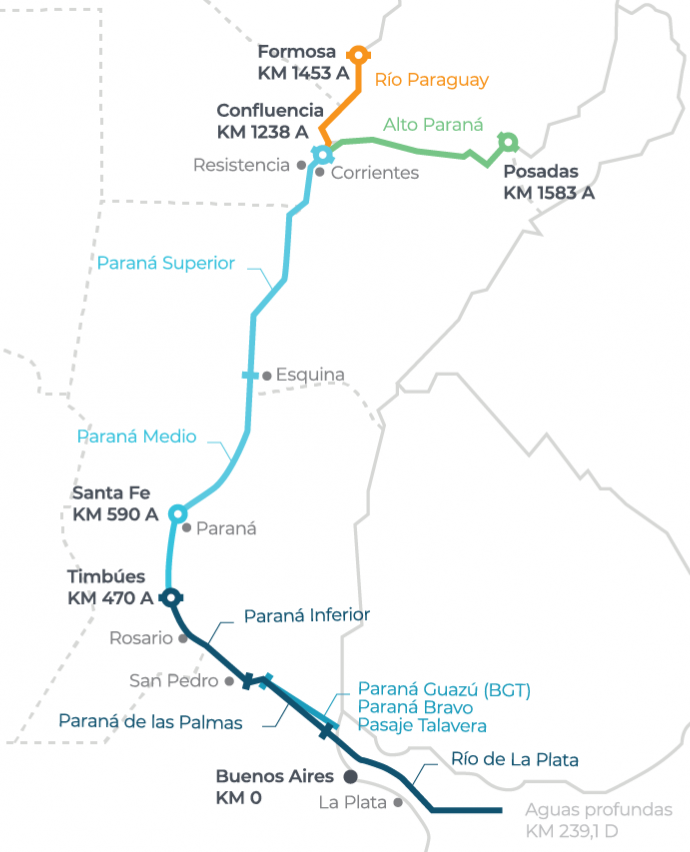
\includegraphics[width=0.5\linewidth]{figures/2025_mapa_vnt_extendida_tramos_profundidades_abril.png}
    \caption{The Vía Navegable Troncal (VNT) and the location of the Paraná Guazú in it \autocite{NavegableTroncal2025}}
    \label{fig:VNT}
\end{figure}

\section{Classification of Rio Paraná}

Rivers can be described and classified in different ways. This classification can be linked to several factors such as age, colour or seasonality. 

\subsection{The Age Classification of a River}
Based on the development of the channel stage of a river, it can be labeled as youthful, mature or old age.  \autocite{davisGeographicalCycle1899}
Applying this to the Rio Paraná makes it a complicated choice since the river is so long that it possesses features linked to each age label at distinct locations. therefore, it would be wiser to divide the Rio Paraná in three parts: upper, middle and lower Paraná. A youthful channel can be recognized through rapid flow, significant erosion, and a steep gradient. All these traits can be attributed to the upper Paraná zone.
Moving on, a mature channel stage of river is in most cases a developed floodplain in the form of loops, called 'meander', and lateral erosion. This is mostly what can be seen in the middle part of the Paraná river.
Lastly, the characteristics of an old age channel are comparable to the lower Paraná river. A wider floodplain, less rapid flow, and Deltas. All of this is explained in \autocite{orfeoParanaRiverArgentine2023}, and can be seen in the following figure from \autocite{lopezweibelSourcesTemporalDynamics2022}.



\begin{figure}[H]
    \centering    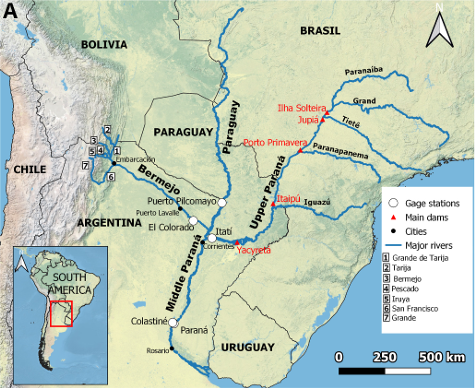
\includegraphics[width=0.5\linewidth]{figures/figure chap 2/map rio parana.png}
    \caption{Rio Paraná Map}
    \label{fig:placeholder}
\end{figure}


From Davis's study it makes sense that all these stages are represented in the total picture of the Paraná river since it is the ninth largest river in the world based on discharge \autocite{lopezweibelSourcesTemporalDynamics2022}.

\subsection{The Colour Classification of a River}
The colour of the river is also another label that can create a distinction. Based on two sets of papers/research  \autocite{furchWaterChemistryAmazon1984}, \autocite{sioliAmazonLimnologyLandscape1984}  Junk 1997, the water in rivers can be described as black, white or clear. The black water river is attributed to the 'leaching of tannins from decayed leaves of adjoining vegetated lands' \autocite{sand-mining-boek}, most comon in Amazonia or in the United States. White waters on the other hand are, contrary to its qualification, usually brown coloured due to the high sediment concentration. Clear water rivers are located in environments with little to no erosion.
Based on the theory and satellite imagery, one can again classify the Rio Paraná in different as a black and white river depending on the zone. The upper Paraná can be considered to be black due to its lack of sediment content, but rich in leaves content. But after the Bermejo river joins the Paraná, the river turns muddy all the way to the sea near Buenos Aires. \autocite{lopezweibelSourcesTemporalDynamics2022}

\begin{figure}[htbp]
    \centering
    \begin{subfigure}[b]{0.48\textwidth}
        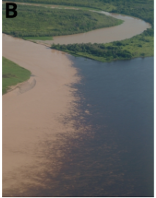
\includegraphics[width=\linewidth, height=5cm]{figures/figure chap 2/Paraguay-Bermejo.png}
        \caption{Confluence of the Paraguay and Bermejo River}
        \label{fig:bermejo}
    \end{subfigure}
    \hfill
    \begin{subfigure}[b]{0.48\textwidth}
        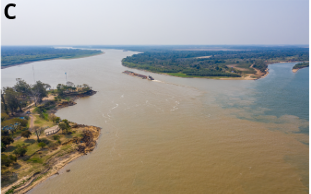
\includegraphics[width=\linewidth, height=5cm]{figures/figure chap 2/Paraguay Parana.png}
        \caption{Confluence of the Paraguay and Paraná River}
        \label{fig:parana}
    \end{subfigure}
    \caption{Confluences of the Paraguay River with the Bermejo (left) and Paraná (right)}
    \label{fig:confluences}
\end{figure}

\subsection{The Seasonal Flow of a River}
The last classification relevant for this study is based on the flow characteristics and water availability. There are once again three types of categories: ephemeral, intermediate and perennial rivers. Ephemeral means that the river flow is not continuously present throughout the calendar year. Perennial rivers are the rivers whose flow is continuous and does not dry up during dry season, unlike the ephemeral rivers. Lastly the intermediate rivers are perennial rivers that dry up in extreme cases of drought.
The Rio Paraná can be considered a perennial river due to its continuous flow over the years \autocite{furchWaterChemistryAmazon1984}, \autocite{sioliAmazonLimnologyLandscape1984}.
 
\section{Mining of the Sand and Types of Dredging in a River}
Due to the need of sand in our society, various techniques have been established to get hold of the sand in the river beds. In this subpart the different dredging techniques will be explained.
For the sake of this study the focus will lie on in stream mining, the extraction of sand and gravel from the active channel of a river \autocite{sand-mining-boek}.

\textit{Bar scalping or skimming}:
This is the most common practice of extraction. It consists of taking away the two thirds of the bar, leaving the top third to minimize the alternation of the river bed initial conditions.

\textit{Dry pit channel mining}:
This method relies on using tools (mechanical or manual) to create a dry pit in which the sand or gravel can be extracted. The state in which the pits are left after extraction act has head cuts, altering the upstream flow during the high seasons.

\textit{Wet pit channel mining}:
Usually, the pit is made in a perennial river, but the effects and damages are the same as for the dry pit channel mining.

\textit{Bar excavation}:
This excavation process happens downstream of the bar, in order to get a hold of the sand and gravel going downstream.

\textit{Instream traps}:
For this excavation method a hole is dug so that the sediment gets caught during high season. This sediment can later be captured when the tides are low again.



\section{The effects of river sand mining}
\subsection{River bed}
As mentioned in the previous section, rivers maintain an equilibrium between erosion, transport, and deposition of sediments. However, instream sand mining can discrupt this balance. This happens through direct disruption of the channel geometry or through so-called incision and related undercutting of banks \autocite{sand-mining-boek}.

The direct disruption of the river bed depends on the type of sand mining technique employed. In the case of pit excavation, the river bed is locally lowered and a so-called 'nick point' is created. With bar skimming the river bed is widened \autocite{sand-mining-boek}. For the remainder of this section, the consequent effects of the local river bed lowering (the nick point) are discussed.

Channel incision causes the nick point to migrate both upstream and downstream. In the case of high flows, due to its shape, the nick point is the point where most erosion occurs. Water plunges over the step and erodes the bed at the base. As flows continue, the drop migrates upstream, a process which is often called head-cutting in literature. On the other hand, a process called 'hungry water' causes downstream migration of the pit \autocite{sand-mining-boek}.

A the mining pit the water level is deeper, which causes the flow velocity to reduce locally. This leads to a decrease in flow energy and thus to more deposited sediment. When the flow leaves the mining area, water levels are shallower again meaning that flow velocity and energy significantly increase. A lot of sediment has been deposited in the nick point, meaning that the water is not using its full sediment carrying capacity anymore. In other words, the water is 'hungry' for sediment and erosion downstream increases \autocite{sand-mining-boek}. 

Through the combined effects of head-cutting and hungry water, the mining pit can extend beyond the initial dimensions caused by direct disruption. This happens in both downstream and upstream directions, as summarized in figure \ref{fig:channelbedeffects}.

\begin{figure}[H]
    \centering
    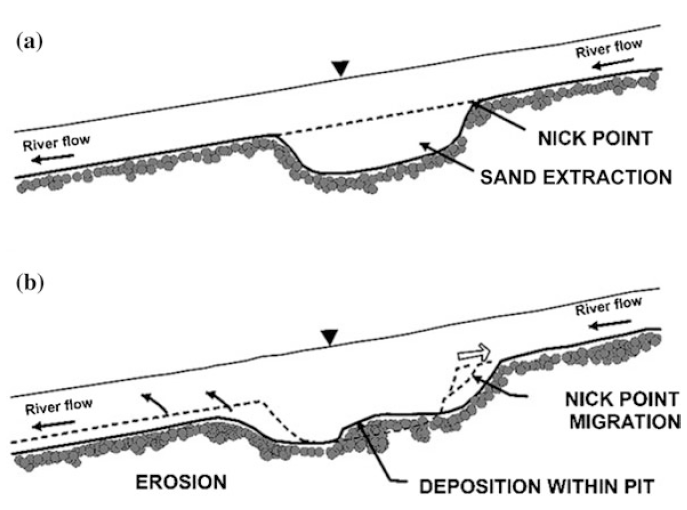
\includegraphics[width=0.75\linewidth]{figures/channelbedeffects.png}
    \caption{a: direct disruption leads to a locally lowered water bed, b: channel incision makes the pit migrate upstream through head cutting and downstream through 'hungry' water \autocite{sand-mining-boek}}
    \label{fig:channelbedeffects}
\end{figure}

\subsection{Sediment}
Previous studies have shown that bed coarsening can occur as a result of sand-mining. Fine particles are removed, leading to a greater concentration of coarse (gravelly) particles. This effect can also be seen upstream \autocite{sand-mining-boek}.

\subsection{Water quality and quantity}
Sand mining can lead to changes in both water quality and quantity. The process of dredging the fine sand stirs fine organic and inorganic particles, thereby increasing the turbidity of the water. This reduces light penetration, which means less photosynthesis and ultimately less organic growth in the water \autocite{sharipEffectsSeasonSand2014}.

As mentioned before, mining pits are often places with significant deposition of particles. Fine, nutrient-rich particles can settle and get trapped in the pits. This then reduces the transport of nutrients from the river to the coastal waters \autocite{sand-mining-boek}.

Concerning the water quantity, the most relevant effects are related to the groundwater: the lowering of the river bed through direct disruption or channel incision can lead to a lower groundwater table. This can lead to settlements or have negative effects on flora and fauna surrounding the river \autocite{rentierEnvironmentalImpactsRiver2022}.

\subsection{Biologic, socioeconomic and infrastructural changes}
The effects of sand mining can be diverse: previous studies have shown negative impacts on biodiversity, including reduced benthic fauna, disrupted fish spawning habitats, and depletion of natural mosquito predators such as dragonflies \autocite{sand-mining-boek}. The socioeconomic effects of mining can vary, in the short-term it often provides employment, income, and government revenue through royalties and taxation. However, in the long-term the operation can cause a reduction in access to clean water and can cause water scracity, especially in dry periods. Additionally, loss of land and access to land together with loss of trees and vegetation can jeapordize the local food security. Finally, infrastructure can be damaged by the lowering of the river bed and/or the groundwater table \autocite{sand-mining-boek}.


\section{Origin of sediment content in Paraná Guazú}

A key step in constructing the sediment balance of the Paraná Guazú, located in the lower Paraná, is to identify the origin of its sediment. As shown in Figure \ref{fig:placeholder}, the lower and middle Paraná receive discharge from three main tributaries: the Bermejo, Paraguay, and upper Paraná rivers. The total average discharge in the middle Paraná is $18,389~\mathrm{m^3/s}$, of which 78\% is supplied by the upper Paraná. \citeauthor{lopezweibelSourcesTemporalDynamics2022} report that the Bermejo contributes only 2\% of this discharge. Nevertheless, the Bermejo is the dominant source of sediment, due to intense erosion in the Andes Eastern Mountain Range within its basin. During the wet season (November to April), multiple tributaries in the basin contribute large sediment flows, accumulating to an annual suspended sediment load of $106 ~\times 10^6$ t per year at El Colorado gauge station. By contrast, sediment supply from the upper Paraná is strongly reduced by hydropower dams that trap material upstream. 

It is interesting to know that the contribution of sediment from the Bermejo to the Paraná is approximately 90\% today, but that this is in fact due to the installation of the Itaipu dam built in 1971. This modification of the sediment voyage cuts a supply of about 50\% compared the initial amount of sediment, this 90\% used to be 56\% of the sediment income before the construction of the dam. This explains us that the involvement of the 

In summary, while the Paraguay and upper Paraná rivers provide most of the fluvial discharge to the downstream delta, the Bermejo River delivers the majority of sediments (\cite{lopezweibelSourcesTemporalDynamics2022}). For this reason, the stretch of river beginning in the Bermejo basin and continuing via the Paraguay and middle Paraná to the Paraná Guazú is of particular importance in this study.  













\chapter{Background Study}
In this part of the report, the research that contributes to the contextualization of the Rio Paraná Guazú will be explained. The goal of the background study is to give the lector an understanding of what theory is used for the later stages of the analysis.

\section{Argentina's waterways}
The Argentine river system can be grouped into three watersheds: the Atlantic watershed, which drain into the Argentine Sea, the Pacific watershed; and, finally the rivers that don't drain into an ocean but flow inland to permanent or seasonal lakes, swamps, or dry sinks. Of these systems, the Atlantic watershed is the most important and includes the Río de la Plata Basin, the Patagonian system, and several smaller rivers in the province of Buenos Aires \autocite{marioe.farberHydrographyArgentina2024}. The Río de la Plata Basin is the most relevant one: it ends in the Río de la Plata estuary and consists of the Paraná, the country's longest river, the Uruguay and their subrivers. The Vía Navegable Troncal (VNT) ends in the Río de la Plata estuary and connects numerous ports to the ocean. Because of this, the VNT is responsible for rougly 80\% of the nation's export \autocite{NavegableTroncal2025}. The Paraná Guazú is part of this main waterway, as can be seen in figure \ref{fig:VNT}.

\begin{figure}
    \centering
    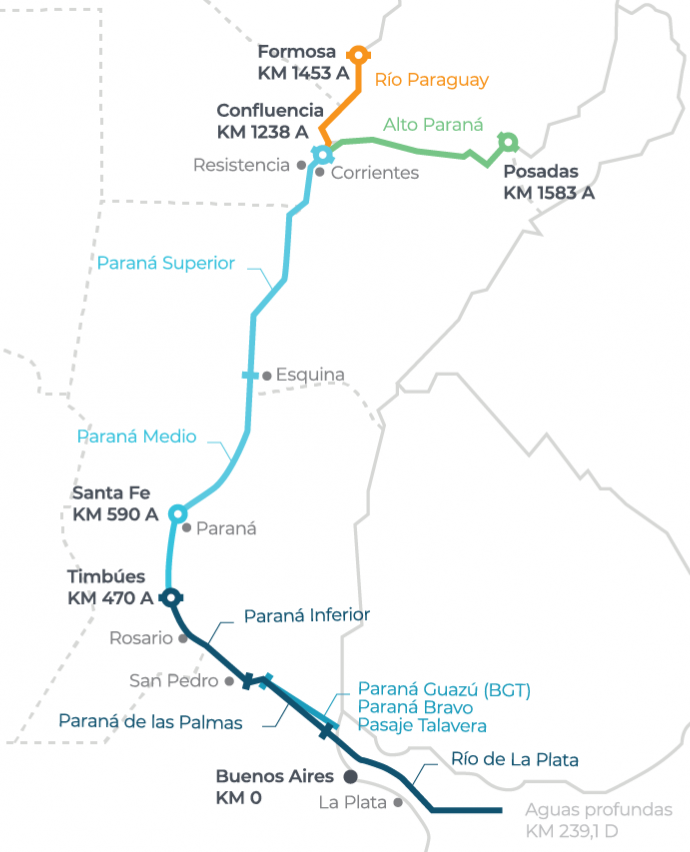
\includegraphics[width=0.5\linewidth]{figures/2025_mapa_vnt_extendida_tramos_profundidades_abril.png}
    \caption{The Vía Navegable Troncal (VNT) and the location of the Paraná Guazú in it \autocite{NavegableTroncal2025}}
    \label{fig:VNT}
\end{figure}

\section{Classification of Rio Paraná}

Rivers can be described and classified in different ways. This classification can be linked to several factors such as age, colour or seasonality. 

\subsection{The Age Classification of a River}
Based on the development of the channel stage of a river, it can be labeled as youthful, mature or old age.  \autocite{davisGeographicalCycle1899}
Applying this to the Rio Paraná makes it a complicated choice since the river is so long that it possesses features linked to each age label at distinct locations. therefore, it would be wiser to divide the Rio Paraná in three parts: upper, middle and lower Paraña. A youthful channel can be recognized through rapid flow, significant erosion, and a steep gradient. All these traits can be attributed to the upper Paraná zone.
Moving on, a mature channel stage of river is in most cases a developed floodplain in the form of loops, called 'meander', and lateral erosion. This is mostly what can be seen in the middle part of the Paraná river.
Lastly, the characteristics of an old age channel are comparable to the lower Paraná river. A wider floodplain, less rapid flow, and Deltas. All of this is explained in \autocite{orfeoParanaRiverArgentine2023}, and can be seen in the following figure from \autocite{lopezweibelSourcesTemporalDynamics2022}.



\begin{figure}[H]
    \centering    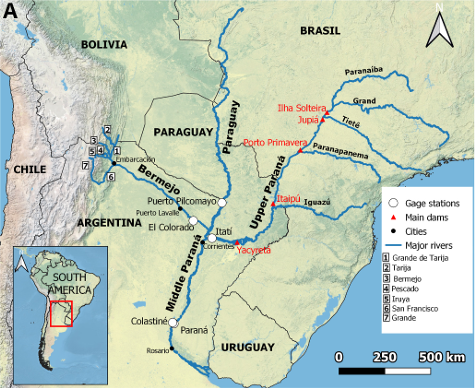
\includegraphics[width=0.5\linewidth]{figures/figure chap 2/map rio parana.png}
    \caption{Rio Paraná Map}
    \label{fig:placeholder}
\end{figure}


From Davis's study it makes sense that all these stages are represented in the total picture of the Paraná river since it is the ninth largest river in the world based on discharge \autocite{lopezweibelSourcesTemporalDynamics2022}.

\subsection{The Colour Classification of a River}
The colour of the river is also another label that can create a distinction. Based on two sets of papers/research  \autocite{furchWaterChemistryAmazon1984}, \autocite{sioliAmazonLimnologyLandscape1984}  Junk 1997, the water in rivers can be described as black, white or clear. The black water river is attributed to the 'leaching of tannins from decayed leaves of adjoining vegetated lands' \autocite{sand-mining-boek}, most comon in Amazonia or in the United States. White waters on the other hand are, contrary to its qualification, usually brown coloured due to the high sediment concentration. Clear water rivers are located in environments with little to no erosion.
Based on the theory and satellite imagery, one can again classify the Rio Paraná in different as a black and white river depending on the zone. The upper Paraná can be considered to be black due to its lack of sediment content, but rich in leaves content. But after the Bermejo river joins the Paraná, the river turns muddy all the way to the sea near Buenos Aires. \autocite{lopezweibelSourcesTemporalDynamics2022}

\begin{figure}[htbp]
    \centering
    \begin{subfigure}[b]{0.48\textwidth}
        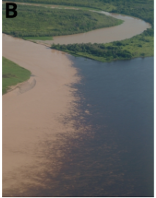
\includegraphics[width=\linewidth, height=5cm]{figures/figure chap 2/Paraguay-Bermejo.png}
        \caption{Confluence of the Paraguay and Bermejo River}
        \label{fig:bermejo}
    \end{subfigure}
    \hfill
    \begin{subfigure}[b]{0.48\textwidth}
        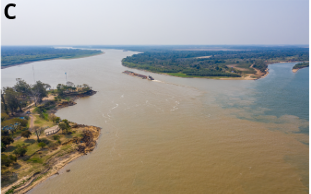
\includegraphics[width=\linewidth, height=5cm]{figures/figure chap 2/Paraguay Parana.png}
        \caption{Confluence of the Paraguay and Paraná River}
        \label{fig:parana}
    \end{subfigure}
    \caption{Confluences of the Paraguay River with the Bermejo (left) and Paraná (right)}
    \label{fig:confluences}
\end{figure}

\subsection{The Seasonal Flow of a River}
The last classification relevant for this study is based on the flow characteristics and water availability. There are once again three types of categories: ephemeral, intermediate and perennial rivers. Ephemeral means that the river flow is not continuously present throughout the calendar year. Perennial rivers are the rivers whose flow is continuous and does not dry up during dry season, unlike the ephemeral rivers. Lastly the intermediate rivers are perennial rivers that dry up in extreme cases of drought.
The Rio Paraná can be considered a perennial river due to its continuous flow over the years \autocite{furchWaterChemistryAmazon1984}, \autocite{sioliAmazonLimnologyLandscape1984}.
 
\section{Mining of the Sand and Types of Dredging in a River}
Due to the need of sand in our society, various techniques have been established to get hold of the sand in the river beds. In this subpart the different dredging techniques will be explained.
For the sake of this study the focus will lie on in stream mining, the extraction of sand and gravel from the active channel of a river \autocite{sand-mining-boek}.

\textit{Bar scalping or skimming}:
This is the most common practice of extraction. It consists of taking away the two thirds of the bar, leaving the top third to minimize the alternation of the river bed initial conditions.

\textit{Dry pit channel mining}:
This method relies on using tools (mechanical or manual) to create a dry pit in which the sand or gravel can be extracted. The state in which the pits are left after extraction act has head cuts, altering the upstream flow during the high seasons.

\textit{Wet pit channel mining}:
Usually, the pit is made in a perennial river, but the effects and damages are the same as for the dry pit channel mining.

\textit{Bar excavation}:
This excavation process happens downstream of the bar, in order to get a hold of the sand and gravel going downstream.

\textit{Instream traps}:
For this excavation method a hole is dug so that the sediment gets caught during high season. This sediment can later be captured when the tides are low again.



\section{The effects of river sand mining}
\subsection{River bed}
As mentioned in the previous section, rivers maintain an equilibrium between erosion, transport, and deposition of sediments. However, instream sand mining can discrupt this balance. This happens through direct disruption of the channel geometry or through so-called incision and related undercutting of banks \autocite{sand-mining-boek}.

The direct disruption of the river bed depends on the type of sand mining technique employed. In the case of pit excavation, the river bed is locally lowered and a so-called 'nick point' is created. With bar skimming the river bed is widened \autocite{sand-mining-boek}. For the remainder of this section, the consequent effects of the local river bed lowering (the nick point) are discussed.

Channel incision causes the nick point to migrate both upstream and downstream. In the case of high flows, due to its shape, the nick point is the point where most erosion occurs. Water plunges over the step and erodes the bed at the base. As flows continue, the drop migrates upstream, a process which is often called head-cutting in literature. On the other hand, a process called 'hungry water' causes downstream migration of the pit \autocite{sand-mining-boek}.

A the mining pit the water level is deeper, which causes the flow velocity to reduce locally. This leads to a decrease in flow energy and thus to more deposited sediment. When the flow leaves the mining area, water levels are shallower again meaning that flow velocity and energy significantly increase. A lot of sediment has been deposited in the nick point, meaning that the water is not using its full sediment carrying capacity anymore. In other words, the water is 'hungry' for sediment and erosion downstream increases \autocite{sand-mining-boek}. 

Through the combined effects of head-cutting and hungry water, the mining pit can extend beyond the initial dimensions caused by direct disruption. This happens in both downstream and upstream directions, as summarized in figure \ref{fig:channelbedeffects}.

\begin{figure}[H]
    \centering
    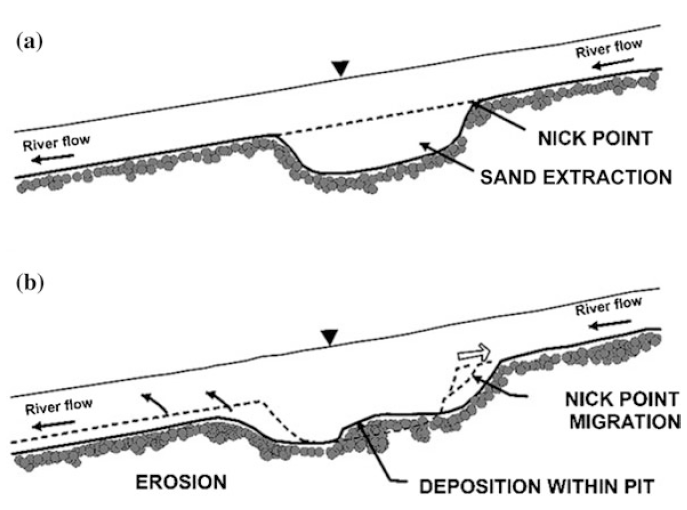
\includegraphics[width=0.75\linewidth]{figures/channelbedeffects.png}
    \caption{a: direct disruption leads to a locally lowered water bed, b: channel incision makes the pit migrate upstream through head cutting and downstream through 'hungry' water \autocite{sand-mining-boek}}
    \label{fig:channelbedeffects}
\end{figure}

\subsection{Sediment}
Previous studies have shown that bed coarsening can occur as a result of sand-mining. Fine particles are removed, leading to a greater concentration of coarse (gravelly) particles. This effect can also be seen upstream \autocite{sand-mining-boek}.

\subsection{Water quality and quantity}
Sand mining can lead to changes in both water quality and quantity. The process of dredging the fine sand stirs fine organic and inorganic particles, thereby increasing the turbidity of the water. This reduces light penetration, which means less photosynthesis and ultimately less organic growth in the water \autocite{sharipEffectsSeasonSand2014}.

As mentioned before, mining pits are often places with significant deposition of particles. Fine, nutrient-rich particles can settle and get trapped in the pits. This then reduces the transport of nutrients from the river to the coastal waters \autocite{sand-mining-boek}.

Concerning the water quantity, the most relevant effects are related to the groundwater: the lowering of the river bed through direct disruption or channel incision can lead to a lower groundwater table. This can lead to settlements or have negative effects on flora and fauna surrounding the river \autocite{rentierEnvironmentalImpactsRiver2022}.

\subsection{Biologic, socioeconomic and infrastructural changes}
The effects of sand mining can be diverse: previous studies have shown negative impacts on biodiversity, including reduced benthic fauna, disrupted fish spawning habitats, and depletion of natural mosquito predators such as dragonflies \autocite{sand-mining-boek}. The socioeconomic effects of mining can vary, in the short-term it often provides employment, income, and government revenue through royalties and taxation. However, in the long-term the operation can cause a reduction in access to clean water and can cause water scracity, especially in dry periods. Additionally, loss of land and access to land together with loss of trees and vegetation can jeapordize the local food security. Finally, infrastructure can be damaged by the lowering of the river bed and/or the groundwater table \autocite{sand-mining-boek}.


\section{Origin of sediment content in Paraná Guazú}

A key step in constructing the sediment balance of the Paraná Guazú, located in the lower Paraná, is to identify the origin of its sediment. As shown in Figure \ref{fig:placeholder}, the lower and middle Paraná receive discharge from three main tributaries: the Bermejo, Paraguay, and upper Paraná rivers. The total average discharge in the middle Paraná is $18,389~\mathrm{m^3/s}$, of which 78\% is supplied by the upper Paraná. \citeauthor{lopezweibelSourcesTemporalDynamics2022} report that the Bermejo contributes only 2\% of this discharge. Nevertheless, the Bermejo is the dominant source of sediment, due to intense erosion in the Andes Eastern Mountain Range within its basin. During the wet season (November to April), multiple tributaries in the basin contribute large sediment flows, accumulating to an annual suspended sediment load of $106 ~\times 10^6$ t per year at El Colorado gauge station. By contrast, sediment supply from the upper Paraná is strongly reduced by hydropower dams that trap material upstream.  

In summary, while the Paraguay and upper Paraná rivers provide most of the fluvial discharge to the downstream delta, the Bermejo River delivers the majority of sediments (\cite{lopezweibelSourcesTemporalDynamics2022}). For this reason, the stretch of river beginning in the Bermejo basin and continuing via the Paraguay and middle Paraná to the Paraná Guazú is of particular importance in this study.  













%\chapter{Stakeholder analysis}
\label{chapter:stakeholders}

In this part of the report, the stakeholders related to Rio Paraná Guazú will be explained. The goal of this stakeholder analysis is to understand the different interests in the region related to sand dredging activities.


\section{Stakeholders}

For the stakeholder analysis, all potentially relevant stakeholders for this project were identified. Some were suggested directly by INA staff, who indicated individuals important for gathering information on the Parana Guazú River. Additional stakeholders were identified through further investigation into relevant contacts. The full list of these stakeholders appears in Table \ref{tab:stakeholders} and will be discussed in the following sections.

\subsubsection{Stakeholders}

\begin{table}[ht]
\centering
\begin{tabularx}{\linewidth}{lX}
\toprule
\textbf{Stakeholder} & \textbf{Role} \\
\midrule
Dredgers & Extraction of sand \\
\midrule
Dredging Companies & Extraction and selling of sand \\
\midrule
Prefectura Naval Argentina & Protects rivers and maritime territory \\
\midrule
Agencia Nacional de Puertos y Navegación & Control of signalling system, dredging, and maintenance \\
\midrule
Ports & Handling and storing of goods \\
\midrule
Fishermen & Local fishermen \\
\midrule
NGOs & Non-profit organizations \\
\midrule
Agua y Saneamientos Argentinos & Delivering water and sewerage services \\
\midrule
Alejo Di Rosio & Filmmaker \\
\bottomrule
\end{tabularx}
\caption{Potential stakeholders}
\label{tab:stakeholders}
\end{table}

\subsubsection{Stakeholders description}

The stakeholders which where given in the overview here above will be shortly described in the following overview. Hereafter, the stakheolders will be described in more detail to get a better understanding of the interests and goals of each specific stakeholder. In Table X an overview of the descriptions is given.

\begin{table}[ht]
\centering
\begin{tabularx}{\linewidth}{lX}
\toprule
\textbf{Stakeholder} & \textbf{Description} \\
\midrule
Dredgers & Extraction of sand \\
\midrule
Dredging Companies & Extraction and selling of sand \\
\midrule
Prefectura Naval Argentina & Protects rivers and maritime territory \\
\midrule
Agencia Nacional de Puertos y Navegación & Control of signalling system, dredging, and maintenance \\
\midrule
Ports & Handling and storing of goods \\
\midrule
Fishermen & Local fishermen \\
\midrule
NGOs & Non-profit organizations \\
\midrule
Agua y Saneamientos Argentinos & Delivering water and sewerage services \\
\midrule
Alejo Di Rosio & Filmmaker \\
\bottomrule
\end{tabularx}
\caption{Potential stakeholders with descriptions}
\label{tab:stakeholders-description}
\end{table}




\subsubsection{Stakeholder interests, problem perception and goal}



\section{Dredgers (LOCAL??)}
The first dominant group of stakeholders are the dredgers.These include the local boats used in the area to extract sand and gravel from the river. There are several different types of dredgers ranging from small independent boats, to groups of small boats that work for the same employer (ARENEROS??), or big extracting ships commonly referred to as 'hoppers'. In the area of interest, the Paraná Guazú from Ibicuy to Brazo Largo, the most common dredgers are: (ARENEROS, INDEPENDENT BOATS). 

Currently there are 2 active boats in the zone of the Rio Paraná Guazú of interest, and (QUITE A LOT MORE IN IBICUY?? FROM INTERVIEW), as mentioned in the previous Chapter. (DREDGING ACTIVITY AANGEVEN WELKE BOTEN, MAPS MET HEEN EN TERUG REIS, DATA , ETC)

Their interest in the Rio Paraná Guazú is to extract the sand in locations of the river that are shallow since they do not possess any technology to mine the sand from deep. Once this water mixed sand is lifted onto the boat, they transport it to the nearest ports, Ibicuy or Brazo Largo. They sell their sand to the highest bidder which can be for (PURPOSES FROM INTERVIEW).


\section{BIG Dredging Companies?}
because they buy the sand and employ the areneros?
The Dredging companies active in the Rio Paraná Guazú are :
(EERST KIJKEN OF YPF, JAn de NUl, etc hierbij kan worden betrokken of niet)


\section{Prefectura Naval Argentina}
The Prefectura Naval Argentina (PNA), is the National Naval Prefecture of the Rio Paraná. Therefore, they are also active in the Paraná Guazú and our area of surveillance. 
It is in their interest to protect the Rio Paraná Guazú from criminal activities. These can 

\section{Agencia Nacional de Puertos y Navegación}
The Agencia Nacional de Puertos y Navegación (ANPYN), or the National Agency of Ports and Navigation, was created on January 6, 2025 by a merger of the Undersecretariat of Ports, Waterways and Merchant Marine and the General Port Administration. Since then, the agency has taken over the tasks of the two former entities and is now responsible for policies concerning ports, waterways and river and maritime transport. As such, keeping the Vía Navegable Troncal (VNT), Argentina's main waterway, navigable for ships is an important task for the agency. To achieve this, they regulate dredging and sand mining contracts and oversee compliance with the relevant regulations .

\section{Ports}
In the researched area there are two strategic port locations that play a key role in the sand extraction.

\subsection{Guazú}
?
\subsection{Ibicuy}
?

\section{Fishermen}
Fischermen is another stakeholder group relevant for this study. The Rio Paraná Guazu is used by a lot of people for its high concentration of fish. 

The artisanal fisheries play an economic role as most of the harvest is sold to middlemen, freezing plants, or in informal markets. Of particular interest are long-range migratory species such as sábalo (Prochilodus lineatus), surubí (Pseudoplatystom corruscans, P. reticulatus), boga (Megaleporinus obtusidens), pacú (Piaractus mesopotamicus), and dorado (Salminus brasiliensis), that support artisanal, recreational, and subsistence fisheries, as observed in other large neotropical rivers, \autocite{assessment of sabalo}, \autocite{fishers' knowledge}

the fischermen in the region of interest are mostly independent. Even though there exists such thing as fischermen associations in the Rio Paraná Guazú, they are not influencial 



\section{NGO's}
even wachten tot ik een nice milieu organisatie vind.

\section{Agua y Saneamientos Argentinos}
Even wachten tot interview met hun, kijken of ze wel relevant zijn


\section{Filmmaker}

When researching for the stakeholders which were relevant for the analysis. We stumble upon an article on a film that was made on the Parana-Paraguay waterway. In this documentary, the focus is on the impact of the trade happening on the Parana-Paraguay waterway. The documentary is made by filmmaker Alejo Di Risio, who was contacted through journalist Matias Avramow for any additional information about stakeholders and business related to the waterway.

 % Create file to add

\chapter{Conclusion}
\label{chapter:conclusion}

\emph{A conclusion...}


%% Prevent urls running into margins in bibliography
\setcounter{biburlnumpenalty}{7000}
\setcounter{biburllcpenalty}{7000}
\setcounter{biburlucpenalty}{7000}

%% Add bibliography
\printbibliography[heading=bibintoc,title=References]

%% ----------------------------------------------------------------------
%%    Appendix (Letters for chapters)
%% ----------------------------------------------------------------------

\appendix

\chapter{Source Code Example}
%\label{chapter:title}

\emph{Adding source code to your report/thesis is supported with the package {\normalfont\texttt{listings}}. An example can be found below. Files can be added using {\normalfont\texttt{\textbackslash lstinputlisting[language=<language>]\{<filename>\}}}.}

\begin{lstlisting}[language=Python]
"""
ISA Calculator: import the function, specify the height and it will return a
list in the following format: [Temperature,Density,Pressure,Speed of Sound].
Note that there is no check to see if the maximum altitude is reached.
"""

import math
g0 = 9.80665
R = 287.0
layer1 = [0, 288.15, 101325.0]
alt = [0,11000,20000,32000,47000,51000,71000,86000]
a = [-.0065,0,.0010,.0028,0,-.0028,-.0020]

def atmosphere(h):
    for i in range(0,len(alt)-1):
        if h >= alt[i]:
            layer0 = layer1[:]
            layer1[0] = min(h,alt[i+1])
            if a[i] != 0:
                layer1[1] = layer0[1] + a[i]*(layer1[0]-layer0[0])
                layer1[2] = layer0[2] * (layer1[1]/layer0[1])**(-g0/(a[i]*R))
            else:
                layer1[2] = layer0[2]*math.exp((-g0/(R*layer1[1]))*(layer1[0]-layer0[0]))
    return [layer1[1],layer1[2]/(R*layer1[1]),layer1[2],math.sqrt(1.4*R*layer1[1])]
\end{lstlisting}

\chapter{Reflection and Task Division}
\label{chapter:Reflection and Task Division}

\section{Reflection}
Throughout our MDP project, our group maintained a collaborative approach to ensure efficiency and good communication. To optimize our workflow, we divided the team into two groups of three: one attended INA on Mondays, while the other went on Wednesdays. This allowed us to maintain a consistent presence at INA while ensuring all members had equal access to resources and stakeholders. On Tuesdays, the entire group worked at the Boskalis office, creating a productive team alignment since we had access to a blackboard. The remaining days were dedicated to remote work, where we operated as a unified group from home, adhering to a standard internship schedule from 9 to 17, in the living room on the dinner table.


Communication with our supervisors primarily took place during our office days at INA. Outside these days, we relied on digital platforms such as Teams, WhatsApp, and email to stay connected and address any questions or updates. This hybrid approach ensured continuous guidance and support, regardless of our physical location.


Deadlines were managed proactively through a planning process, or spontaneous meetings outside working hours which we developed as a group at the outset of the project. Each milestone and task was discussed collectively, allowing us to give out responsibilities effectively and ensure everyone was aligned with the project’s main question. This approach not only kept us on track but also encouraged open communication and constructive debates during group work sessions.


Overall, the combination of in-person and remote collaboration, clear communication channels, and a well-structured planning process contributed to a productive and cohesive team dynamic. Our ability to adapt to different working environments—whether at INA, Boskalis, or remotely—strengthened our multidisciplinary integration and ensured the successful fulfillment of project requirements.

\section{Task Division}

Throughout the ten weeks of the project every student of the MDP385 Group has actively contributed to the project. 
The contributions have been allocated to one of several students per Chapter in the Report. This can be seen in the Table below.


\begin{table}[H]
    \setlength\extrarowheight{4pt}
    \centering
    \caption{Distribution of the workload}
    \label{tab:taskdivision1}
    \begin{tabularx}{\textwidth}{lXX}
        \toprule
        & Task & Student Name(s) \\
        \midrule
        & Summary & All \\
        Chapter 1 & Introduction & All \\
        \midrule
        Chapter 2 & Background Study & \\
        2.1 & Argentina’s waterways & Victor \\
        2.2 & Classification of Rio Paraná & Victor \\
        2.3 & Origin of sediment content in Paraná Guazú & Jasper \\
        2.4 & Mining of the Sand and Types of Dredging in a River & Niek \\
        2.5 & The effects of river sand mining & Niek \\
        \midrule
        Chapter 3 & Methodology & \\
        3.1 & Data collection & Jasper Stefan\\
        3.2 & Field study & Victor Laurens \\
        3.3 & Setting up the Sediment Balance & Stefan \\
        3.4 & Bank Erosion & Victor \\
        3.5 & Multidisciplinary approach &  Mike \\
        \midrule
        Chapter 4 & Stakeholders & \\
        4.1 & Stakeholder analysis & Mike Niek\\
        4.2 & Interview results & Niek \\
        4.3 & Updated stakeholder analysis & Mike \\
        \midrule
        Chapter 5 & Sand extraction & \\
        5.1 & Dredging activities & Laurens \\
        5.2 & Dry sand mining & Niek Laurens\\
        \midrule
        Chapter 6 & Hydrodynamical and sedimentary analysis & \\
        6.1 & Effect of tides and waves on the water level & Victor\\
        6.2 & Hydrodynamic data & Jasper Stefan\\
        6.3 & Sediment transport & Stefan \\
        6.4 & Field work measurements & Laurens\\
        6.5 & Hydrodynamic effects on the River Banks & Victor \\
        \bottomrule
    \end{tabularx}
\end{table}

\begin{table}[H]
    \setlength\extrarowheight{4pt}
    \centering
    \caption*{}
    \label{tab:taskdivision2}
    \begin{tabularx}{\textwidth}{lXX}
        \toprule
                Chapter 7 & Delft3D Model & Jasper Stefan\\
        \midrule
        Chapter 8 & Mitigation Strategies & \\
        8.1 & Nature-based Solutions for bank erosion & Laurens \\
        8.2 & Structural Solutions for bank erosion & Mike \\
        8.3 & Nature-based Solutions for dry sand mining & Niek \\
        \midrule
        Chapter 9 & Discussion & Niek \\
        \midrule
        Chapter 10 & Conclusion and recommendations & All \\
        \midrule
        Appendix A & Codes?? & Mike \\
        Appendix B & Reflection and Task Division & Victor \\
        Appendix C & Safety Assessment & Laurens \\
        Appendix D & Unprocessed interview results & Niek \\
        Appendix E & Laboratory Data & Victor Laurens \\
        Appendix F & Hydrodynamic Satellite Data & Victor \\
        Appendix G & ADCP Results & Stefan Jasper\\
        \midrule
        & Document Design and Layout & All \\
        \bottomrule
    \end{tabularx}
\end{table}

\section{Fieldwork Tasks and Planning}

For the fieldwork, different tasks were assigned, which were not included in the task division table. 
Therefore, the pdf document used during the trip has been translated and put down below.
Note that repeated info such as list of stakeholders and interview questions have not been included.

\subsubsection{Wednesday (DAY 1)}
8:00 Departure from BA (Group 1 and Group 2)
Group 1: Stefan, Victor, Jasper
Group 2: Niek, Laurens, Mike
Group 1: Boat Group
10:00 Arrive at Recreo Keidel, drop off and set up camping gear, and pay (250,000 ARS).
11:00 Meet the fisherman’s boat with Martin (give money for boat).
11:30 Prepare the boat for Thursday (confirm time, location, and details).
12:30 Prepare equipment and ask for explanations to avoid losing time.
Lunch
Drive to stakeholders (45 min) east of RN12 bridge.
14:30 Camping La Torre
15:30 Yacht Club Guazú
Drive back to camping (30 min)
16:30 Arrive back at camp or similar.
Group 2: Stakeholders (car with marina)
Proposal: Drive directly to Ibicuy to conduct the first interviews and avoid traveling back and forth from the campsite (2.5-hour drive from 9 de Julio Avenue).
Arrive around 10:30–11:00.
Morning interviews if possible, otherwise, schedule after appointments:

Camping Los Abuelos
Camping Boca Del Pavón
Club de Pescadores Olivos (Ibicuy branch)
If time allows, visit the northern end of the area:
Camping El Islerito (above Ibicuy port, quite remote)
Lunch
13:00 Meeting with Ibicuy Port Manager
15:00 Meeting with Ibicuy Mayor
Drive back to camping (1 hour 15 min)
17:00 Arrive back at camp or similar. If earlier, conduct additional interviews around Puerto Guazú.
Ask Marina to translate live if recording is not allowed.


\subsubsection{Thursday (DAY 2)}
Group 1: Stefan, Jasper, Niek
Group 2: Laurens, Mike, Victor
Group 1: Boat Group
Start as early as possible to avoid returning late.
8:00–9:00 Board the boat.
Measurements:

Cross Sections 1, 2, 3 around the dredging point
Discharge measurement with SonTek M9
Flow velocity with radar
Bed load with metal digging tool
Sediment concentration with bottles
Soil sample with excavator
Record notes and trajectory in Locus Map for later GIS import and report inclusion.
Lunch on the boat.
Switch tasks during lunch if possible.
Return to camping by 18:00.

Group 2: Stakeholders
Stay near Guazú for stakeholders; possibly depart at 8:30 (50 min drive to Puerto Guazú).
9:30 Arrive in Puerto Guazú.

9:30 Camping Iponá Guazú
10:00 El Molino Camping
10:30 Port Guazú (Do we have a meeting scheduled, or should we improvise?)
11:00–12:00 Visit Arenera del Guazú to observe small dredging vessels.
Lunch
Drive to Constanza (30 min).
At two small harbors (Constanza and another):
14:00 Camping El Amanecer (near two small harbors)
15:00 Camping La Blanqueada
15:30 Oasis Guazú
Drive back to camping (1 hour).


\subsubsection{Friday (DAY 3)}
Group 1: Laurens, Mike, Victor
Group 2: Jasper, Stefan, Niek
Group 1: Boat Group
8:00–9:00 Board the boat.
1–1:30 Travel to Cross Section 4 in Ibicuy.
Measurements:

Cross Section 4 in Port Ibicuy
Discharge measurement with SonTek M9
Flow velocity with radar
Bed load with metal digging tool
Sediment concentration with bottles
Soil sample with excavator
Record notes and trajectory in Locus Map for later GIS import and report inclusion.
Lunch on the boat.
1–1:30 Travel to Cross Section 4 in Ibicuy.
16:30 Return to camp (estimated by Martin).

Group 2: Stakeholders
9:00 Pack up camping gear and check out.
Reserve day for stakeholders or redistribute tasks, e.g., visit the east side of Puerto Guazú if Group 1 couldn’t on Wednesday. Alternatively, summarize stakeholder findings.
Or:
Drive 45 min east of RN12 bridge.
14:30 Camping La Torre
15:30 Yacht Club Guazú
Drive back to camping (30 min).
Groups 1 and 2:
Drive back to Buenos Aires together, dropping off at strategic locations for faster travel home.
1.5–2 hours drive back to BA.
19:00 Arrive home or similar.
%
\chapter{Safety assessment}

This appendix presents the risk assessment associated with the procedures that will be conducted in the fieldwork as part of the multiple discipline project titled "Delft University of Technology Sediment Balance in a Sector of the Paraná Guazú River"

\section{Risk Assessment: Fieldwork}

\subsection{Hazard Identification}
This fieldwork involves extensive activities both on and around the water, which inherently present a variety of safety and health hazards. Working in such environments requires continuous awareness and precautionary measures to protect all members of the research team.
The most severe hazard associated with water-based fieldwork is the risk of drowning. This can occur as a result of falling from boats, working on unstable or slippery riverbanks, or being caught in strong currents. Proper use of life jackets, safe boarding procedures, and clear communication within the group are therefore essential preventive measures.

In addition to the immediate risks of drowning, environmental and weather-related factors can also impact safety. High temperatures and prolonged exposure to the sun may cause heat stress, dehydration, or sunburn, while sudden changes in weather—such as heavy rainfall, thunderstorms, or strong winds—can rapidly increase danger on the water. Adequate protective clothing, hydration, and weather monitoring should be part of the fieldwork routine.

Contact with surface water may also expose researchers to biological hazards. Natural water bodies can contain bacteria, parasites, or other microorganisms that cause skin infections or gastrointestinal illness. Wearing waterproof gloves, avoiding direct contact with open wounds, and practicing proper hygiene (e.g., hand washing or use of disinfectants after fieldwork) are effective ways to reduce these risks.
Another aspect to consider is the safe handling of mechanical and sampling equipment. Working with pumps, sieves, augers, or motorized boats requires attention to mechanical hazards such as entanglement, cuts, or equipment malfunction. Ensuring that all equipment is well maintained and operated only by trained individuals minimizes these dangers.

Finally, the natural environment itself may present additional threats from wildlife. These can range from sharp shells or stinging organisms in the water, to insect bites, snakes, or other animals encountered near the riverbank. Using appropriate footwear, insect repellent, and maintaining awareness of the surroundings can help prevent injuries or allergic reactions.


\subsection{Risk Assessment}
The risks associated with this fieldwork vary both in their likelihood of occurrence and in the severity of their potential consequences. Understanding this balance is essential for prioritizing safety measures and ensuring that all critical hazards receive appropriate attention and control.

The risk of drowning, although assessed as having a low likelihood under normal operating conditions, carries extremely severe consequences should it occur. Because of the potentially fatal outcome, this hazard remains a critical concern and must always be treated with the highest level of precaution. Preventive actions such as the mandatory use of life jackets, maintaining clear safety protocols during boat operations, and ensuring all participants are trained in emergency procedures are therefore non-negotiable components of field safety.

Risks arising from weather conditions are more likely to occur and can vary throughout the day. The likelihood of exposure to heat, sun, or sudden changes in weather is considered relatively high, while the potential consequences—ranging from mild heat stress to temporary work interruptions—are moderate. Nevertheless, such risks should be actively mitigated through measures including weather monitoring, adequate rest and hydration, the use of sun protection, and flexible planning to avoid dangerous conditions.

Biological hazards, such as exposure to bacteria or other pathogens present in the water, are generally considered to have a low likelihood of occurrence if proper hygiene and protective measures are followed. However, the consequences of such exposure can be significant, including illness or infection. For this reason, it is vital that all team members remain aware of these hazards and adhere strictly to personal protection and sanitation guidelines, such as using gloves, avoiding contact with open wounds, and washing hands thoroughly after field activities.

Finally, hazards related to mechanical equipment—such as cuts, entanglement, or mechanical malfunction—are assessed as having a low likelihood in this specific fieldwork setting. Their potential consequences are moderate, primarily involving minor injuries or temporary disruption of operations. Routine maintenance, proper training, and adherence to safe operating procedures are sufficient to keep this risk at an acceptable level.


\subsection{Control Measures}
To minimize potential risks during fieldwork, it is essential that all participants make consistent and appropriate use of personal protective equipment (PPE). Key items include life jackets when working on or near the water, sturdy footwear with sufficient grip to prevent slipping on wet or uneven surfaces, and protective gloves when handling tools, equipment, or biological materials. The type of gloves may vary depending on the specific task—ranging from waterproof gloves for wet environments to cut-resistant gloves when working with sharp instruments.

Equally important is ensuring that every team member is fully aware of the hazards present in the field environment. To achieve this, a comprehensive safety briefing must be conducted before any field activities begin. During this briefing, all risks, safety procedures, and emergency response protocols should be clearly explained, allowing participants to understand both their individual responsibilities and the collective safety measures of the group.

Maintaining proper hygiene also plays a crucial role in minimizing biological risks. Regular handwashing, particularly before eating or after contact with river water, significantly reduces the likelihood of bacterial or parasitic infections. The availability of clean water, disinfectant wipes, or alcohol-based sanitizers should therefore be ensured at all times.

In the event of an emergency, effective communication is vital. All team members must be reachable at short notice to enable rapid coordination and response. For this reason, everyone should carry a charged mobile phone at all times. A clear communication plan—including designated contact persons and emergency numbers—should be established before fieldwork begins.

By combining the proper use of PPE, strong situational awareness, good hygiene practices, and reliable communication systems, the risks associated with water-based fieldwork can be significantly reduced, ensuring a safe and efficient working environment for all participants. % Create file to add

\end{document}
